\documentclass[12pt,a4paper]{article}
\usepackage{titlesec}
\usepackage{fancyhdr}
\usepackage{titlesec}
\newcommand{\sectionbreak}{\clearpage}
\usepackage{apacite}
% !TEX TS-program = pdflatex
% !TEX encoding = UTF-8 Unicode
\usepackage[utf8]{inputenc} % set input encoding (not needed with XeLaTeX)
\usepackage{graphicx} % support the \includegraphics command and options
\usepackage{pdfpages}

%%% PACKAGES
\usepackage{booktabs} % for much better looking tables
\usepackage{array} % for better arrays (eg matrices) in maths
\usepackage{paralist} % very flexible & customisable lists (eg. enumerate/itemize, etc.)
\usepackage{verbatim} % adds environment for commenting out blocks of text & for better verbatim
\usepackage{subfig} % make it possible to include more than one captioned figure/table in a single float
\usepackage[toc,page]{appendix}
\usepackage{url}

\makeatletter
\renewcommand\paragraph{%
    \@startsection{paragraph}{4}{0mm}%
       {-\baselineskip}%
       {.2\baselineskip}%
       {\normalfont\normalsize\bfseries}}
\makeatother

\hbadness=99999

%header and footer settings
\pagestyle{fancyplain}
\fancyhf{}
\renewcommand{\headrulewidth}{0.5pt}
\renewcommand{\footrulewidth}{0.5pt}
\setlength{\headheight}{15pt}
\fancyhead[L]{Jacob Barrow - 40337360}
\fancyhead[R]{ SOC10101 Honors Project}
\fancyfoot[L]{}
\fancyfoot[C]{\thepage}


\usepackage{listings}
\usepackage{xcolor}

\definecolor{codegreen}{rgb}{0,0.6,0}
\definecolor{codegray}{rgb}{0.5,0.5,0.5}
\definecolor{codepurple}{rgb}{0.58,0,0.82}
\definecolor{backcolour}{rgb}{0.95,0.95,0.92}

\lstdefinestyle{mystyle}{
    backgroundcolor=\color{backcolour},   
    commentstyle=\color{codegreen},
    keywordstyle=\color{magenta},
    numberstyle=\tiny\color{codegray},
    stringstyle=\color{codepurple},
    basicstyle=\ttfamily\footnotesize,
    breakatwhitespace=false,         
    breaklines=true,                 
    captionpos=b,                    
    keepspaces=true,                 
    numbers=left,                    
    numbersep=5pt,                  
    showspaces=false,                
    showstringspaces=false,
    showtabs=false,                  
    tabsize=2
}

\lstset{style=mystyle}


\newif\iffluff

\flufffalse

%this starts the document
\begin{document}

\input{./Dissertation-Title.tex}
\iffluff
\input{./Dissertation-Dec.tex}

\pagebreak
\input{./Dissertation-DP.tex}
\pagebreak
\fi

\begin{abstract}
% fill the abstract in here
\end{abstract}
\pagebreak

\tableofcontents % is generated for you
\newpage

\iffluff
\listoftables
\newpage

\listoffigures
%you may have captions such as equations, listings etc they should all appear as required
%these are done for you as long as you use \begin{figure}[placement settings] .. bla bla ... \end{figure}
\newpage

\section*{Acknowledgements}
Insert acknowledgements here
\newpage
\fi

\section{Introduction}

\subsection{Project Outline}
The project will consist of a range of deliverables and milestones.
 
\paragraph{Background Research}
A literature review will be undertaken to provide context to the project and define its scope

\paragraph{Data collection}
In order to provide the algorithm with articles to classify, a dataset is required. It will be sourced from a range of publishers, and ideally cover a large timescale to allow trends to be identified.

\paragraph{Data Labelling}
A raw dataset can be made more valuable by creating a training set from it. This will be a small subsection of the articles that volunteers will label with their perception of the incongruence.

\paragraph{Algorithm Creation}
Once a dataset is generated and labelled, the algorithm to classify the articles can be implemented. 

\paragraph{Analysis}
The algorithm will create a range of datapoints that can be analysed. Trends will be spotted in the dataset used, and comparisons made with different implementations of the algorithm.

\paragraph{Discussion}
...


\pagebreak

\section{Background Research}
\subsection{Types of Incongruence}
\citeA{chesney2017} talks about the differences between clickbait, fake news, sensationalism and incongruent headlines.

\subsubsection{Clickbait}
\citeA{potthast2016} define clickbait as a kind of "web content [...] designed to entice its readers into clicking an accompanying link". Clickbait uses exagerated language, outright fake information and can be accompanied by graphics designed to entice a reader. Figure \ref{fig:clickbait} shows an example of clickbait, sourced from a Natural Health website \footnote{\url{https://naturalon.com/}}.

\begin{figure}[h!]
  \includegraphics[width=\linewidth]{images/clickbait.png}
  \caption{Several clickbait articles in a 'chum box'}
  \label{fig:clickbait}
\end{figure}

\citeA{mahoney2015} terms a collection of clickbait stories as a 'chum boxes' - chum being dead fish used as bait for other fish. \citeauthor{mahoney2015} goes on to examine how clickbait uses pyschological methods to manipulate, an how they can have an unconcious effect on an individual.

\subsubsection{Fake News}
\citeA{allcott2017} defines fake news to be "news articles that are intentionally and verifiably false, and could mislead readers". For example, a fake news conspiracy theory claimed that a pizzeria, Comet Ping Pong, in Washington ran a child sex ring in its basement. Figure \ref{fig:fakenews} shows a news article from 2016 from Your News Wire\footnote{\url{https://archive.is/YTk3n}} (now News Punch).


\begin{figure}[h!]
  \includegraphics[width=\linewidth]{images/fakenews.png}
  \caption{A fake news story}
  \label{fig:fakenews}
\end{figure}


This lead to a man walking into Comet Ping Pong with an assult rifle and firing several shots. The restauraunt's owner and staff also recieved several death threats \cite{lopez2016}. 

\citeauthor{allcott2017} go further in their definition, and give the following sub-categories for fake news: satire, parody, fabrication, manipulation, advertising and propoganda. While the intention of satire and parody is not to decieve but to criticise, the other classifications have more subversive aims, such as misinforming people or gaining as many clicks as possible.

\subsubsection{Sensationalism}
\citeA{molek2013} defines sensationalism as "a specific discourse strategy  aimed  at  channeling  audience's  attention,  which  may  well  be  resorted  to  by  both  popular and quality outlet". They suggest that media fails to provide important and valuable news, in preference for that which is superfical and quick-paced.


Below are examples of sensationalised headlines, sourced from The Sun:

\begin{itemize}
	\item DOOMSDAY DISEASE FEARS Terrorists could turn ‘sniff and die’ virus that kills victims in 24 hours into a BIO-WEAPON
	\item SPICE UP YOUR LIFE Chilli and ginger ‘slash the risk of cancer – stopping tumours growing’
	\item JAB DEBATE As Melinda Messenger slams the HPV jab the parents of two teenagers blame their daughters’ ‘paralysis on vaccine’
	\item 'I KNOW WHO KILLED JONBENET' Juror from the JonBenet Ramsey case gives sensational interview revealing he ‘knows who killed six-year-old’
	
\end{itemize}

These headlines use dramatic language ('slams', 'sensational', 'slash') to evoke a sense of urgency and excitement in the reader, urging them to click through to the rest of the article. Unlike clickbait headlines, information is not withheld but rather dramatised - while the aim is still to get as many clicks as possible, this is achieved through different means.

This sensationalism is intended to provoke and entertain, at times at the expense of accuracy \cite{chesney2017}.

\subsubsection{Project scope}
This project will not consider fake news - by it's nature, the entirity of a fake news article will be false, not just the headline. Therefore, in order to determine whether an article is fake, external sources would have to be consulted. Creating an algorithm for the truth, while an open problem in computer science\footnote{\url{https://www.youtube.com/watch?v=leX541Dr2rU}}, is considered out of the scope of this project.

Instead, this study will seek to evaluate to what extent a headline represents an article's body. This could identify sensationalism, over exaggerated news stories and potentially some types of clickbait.

\subsection{Impact of Incongruence}
\subsubsection{Manufacturing Outrage}
\subsubsection{}
For people who read beyond the headlines - \citeA{ecker2014} ran experiments that investigated how headlines effect the processing of the facts in news "Information that is initially accepted as valid but is later foundto be incorrect can have a persistent influence on people’s memoryand reasoning"


\subsection{Existing Approaches}
A range of studies have already considered several aspects of this project.

\citeA{manjesh2017} used Natural Language Processing (NLP) to identify 'clickbait' headlines, however they did not consider the headline's relationship to the article.


\pagebreak

\section{Methodology}
\subsection{Data Collection}
In order to create an algorithm to detect incongrouence in news articles, first news articles have to be collected. While there are already existing datasets, they tend to be incomplete, out of date, or in innacessiable formats, as they've been made to tackle different problems.

To overcome these obstacles, a bespoke dataset needs to be created that can be classified and analysised by an NLP algorithm.

\subsubsection{Attributes}
Before collecting the data, it's important to decide what form it'll take and what attributes will be stored.

As the aim of the project is to identify incongruence between an articles headline and body, these two attributes will be included in the dataset. In order to identify trends and allow for further analysis, the article's date of publication and the publisher (e.g. BBC, The Guardian, etc.) will also be stored.

Collection could have gone further and retained the articles category (e.g. 'politics', 'sport' etc.), but different publishers categorise articles in different ways - for instance, the BBC has a combined 'Science and Environment' category, whereas The Guardian splits these into two distinct categories. Additionally, similar news articles can be filed under different categories, depending on the publisher. As this project's focus is on the article's content, and not categorisation, it can be considered out of scope to investigate the interplay between different publisher's approach to categorising articles.

\subsubsection{Sources}
The Independent is one of the only online publishers to make available their entire archives. Using the methods mentioned in Section \ref{obtaining-data}, XXX articles were collected, from 2011 to 2020. This 9-year period should prove a useful dataset to analyse a potentially changing landscape in the congruity of news headlines.

The BBC has an 'On This Day' page\footnote{\url{http://news.bbc.co.uk/onthisday}} that has a very select archive from 1950-2005, and analysing these articles could produce some interesting results. However, each of these articles will have been hand-picked (as evidenced by the 'In Context' notes alongside each article), and only represent historic world news events. Therefore, these articles will not be a suitable representation for the average of the time period they are from.

As well as archives, current news was also collected from a range of publishers. A varied range of UK publishers were selected, in order to create a cross

Table \ref{tab:data-sources} shows the full list of data sources collected, as well as the time range they cover and the total records obtained.

\begin{table}[h]
\begin{tabular}{lllll}
\textbf{Publisher} & \textbf{Earliest} & \textbf{Latest} & \textbf{Raw} & \textbf{Cleaned} \\
BBC On This Day & 1950-01-21 & 2005-12-11 & 1857 & 1857 \\
The Independent & 2011-01-01 & XXX & XXX & XXX  \\
BBC & 2019-04-18 & XXX & XXX & XXX  \\
Daily Mail & 2019-09-24 & XXX & XXX & XXX \\
The Guardian & 2020-06-25 & XXX & XXX & XXX \\
Huffington Post & XXX & XXX & XXX & XXX \\
\end{tabular}
\caption{Extents of the data sources collected}
\label{tab:data-sources}
\end{table}

\subsubsection{Obtaining the Data} \label{obtaining-data}
To collect the data, several Python scripts were created. For the daily news, the publishers' various RSS feeds were consulted, and for the archives a more customised approach was taken.

These scripts utilise the BeautifulSoup library to parse each article's webpage and scrape them for the headline, date and body text. As each publisher builds their websites using different design patterns and with different technologies, each script had to be tailor made to fit the page structure. All the scripts used are available in this project's GitHub repository\footnote{\url{https://github.com/jacobbarrow/honours/tree/master/data-collection}}.

In addition, some sites implemented a strict rate-limit on requests - to make a copy of The Independent's archive took around XXX days to complete, scraping one article every 15 seconds. 

\subsubsection{Ethics}
Across a variety of datasets, XXX articles were collected for analysis. This is a substantial amount of data, and represents the work of many individual journalists and news publishers. 

While automated techniques were used to collect the data, everything collected was publically accessiable. In addition, it is legal to make a digital copy of copyrighted data for non-commercial research \footnote{\url{https://www.gov.uk/guidance/exceptions-to-copyright#text-and-data-mining-for-non-commercial-research}}. Even so, care still needs to be taken in the obtainment of the data in order to avoid overloading or altering the regular service of these archives. As mentioned above, requests were rate-limited to avoid inadvertant denial of service attack, and spread out over a long period of time. Additionally, the rolling news was only collected once per day, at midnight, in order to minimise the impact of the scraping.

\subsubsection{Cleaning}
While a bespoke scraper was created for each site, on some articles publishers used different page structures or included certain elements (such as inforgraphics) that the scraper didn't know how to handle. As a result, a portion of the articles in the dataset have erroneous text in them, such as unformatted lists of tweets or social media comments.

When creating the subset of articles for labelling, out of the 300 records 36 (12\%) were corrupt or included content not part of the article's body text. Extrapolating this to the rest of the dataset, this means approximately XXX of the collected articles are 'dirty'.




\subsection{Data Labelling}
\citeA{chesney2017} covers the need for a decent labelled dataset...

Need for labelled data, website design and implementation, crowdsourcing labelling, ethics, analysis of labelled data

\pagebreak
\section{Analysis and Discussion}
\pagebreak
\section{Conclusion}
\pagebreak

\bibliographystyle{apacite}
\bibliography{bibliography}

%you can crate this on a extra tex document just like the title or any other part of the document.
\newpage
\begin{appendices}
\iffluff
\section{Project Overview}
\includepdf[pages=1]{../docs/IPO/IPO}


\section{Second Formal Review Output}
Insert a copy of the project review form you were given at the end of the review by the second marker

\section{Diary Sheets (or other project management evidence)}

\rotatebox{90}{
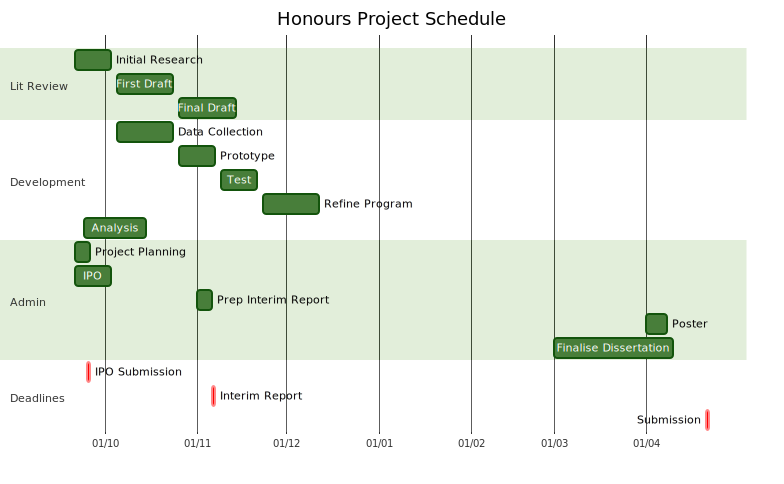
\includegraphics[scale=1,page=1]{../docs/gantt/gantt}
}
\includepdf[pages=1]{../docs/diary/diary}
\includepdf[pages=2]{../docs/diary/diary}
\includepdf[pages=3]{../docs/diary/diary}
\fi
\section{Data Labelling Ethics}


\begin{subappendices}
\subsection{Participant Information Sheet} \label{app:ethics-participant-info}
\includepdf[pages=1]{../docs/ethics/participant-info}

\subsection{RI Approval} \label{app:ethics-approval}
\includepdf[pages=1]{../docs/ethics/RI_Approval}
\includepdf[pages=2]{../docs/ethics/RI_Approval}
\includepdf[pages=3]{../docs/ethics/RI_Approval}
\includepdf[pages=4]{../docs/ethics/RI_Approval}
\includepdf[pages=5]{../docs/ethics/RI_Approval}

\subsection{Example Rating Form} \label{app:rating-form}
\includegraphics[scale=0.5]{../docs/ethics/example_rating-just-form}
\end{subappendices}

\section{Code Listings}
\begin{subappendices}
\subsection{Sentiment Analysis Experiment} \label{app:sentiment-analysis}
\lstinputlisting[language=Python]{../experiments/sentiment-analysis.py}

\subsection{Word Vectorisation Experiment} \label{app:vectorisation}
\lstinputlisting[language=Python]{../experiments/vectorisation.py}
\end{subappendices}

\end{appendices}

\end{document}
